\chapter{Estado del arte}\label{sec:Estado_arte}
\section{Robótica, drones}
Un dron se puede definir como una “aeronave” pilotada de forma remota. El uso de los drones se ha ido instaurando poco a poco en la sociedad; actualmente con sus nuevas mejoras y reducido coste, estos han pasado de una situación en la que era más “amateur” a una función más profesional. En los últimos años han estado cada vez más presentes ya que ofrecen una gran herramienta de trabajo para diferentes sectores tanto comerciales como de seguridad. \newline 

\subsection{Evolución histórica}
La palabra inglesa drone tiene varios significados, aunque en su origen se refiere a los zánganos de las colmenas y al zumbido que emiten. El ruido que se escucha en tierra cuando vuelan a cierta altura estos vehículos recordaba a estos “zánganos” y de ahí que se quedaran con este nombre. Su evolución  proviene sobretodo en el ámbito militar dónde tenían funciones de reconocimiento y permitían tener ventaja en la batalla.\newline 

Los primeros vehículos no tripulados fueron construidos durante la Primera Guerra Mundial . Estos primeros modelos fueron lanzados por catapulta o volados usando radio control. En enero de 1918, el ejército de los Estados Unidos comenzó la producción de torpedos aéreos teleridigidos de forma remota. El modelo que se desarrolló, el Kettering Bug , fue volado con éxito en algunas pruebas, pero la guerra terminó antes de que pudiera desarrollarse más. \newline

\begin{figure}[H]
	\center
	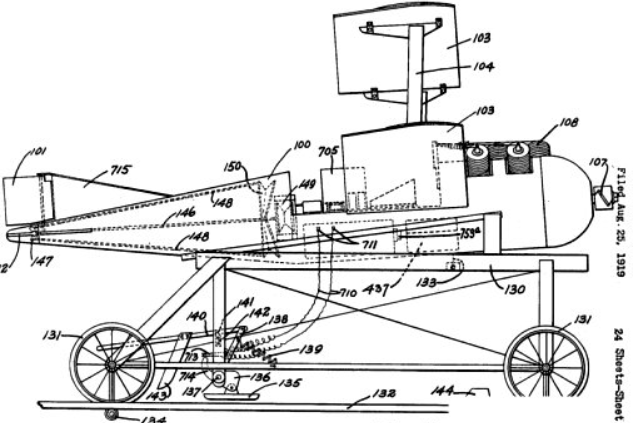
\includegraphics[scale=0.5]{imagenes/EstadodelArte/ketbug.png}
	\caption{Kettering Bug}
	\label{fig:Kettering Bug}
\end{figure}
 

Durante el período de entreguerras continuó el desarrollo y las pruebas de aviones no tripulados. En 1935, los británicos produjeron una serie de aviones controlados por radio para ser utilizados como objetivos con fines de entrenamiento . Los drones controlados por radio también se fabricaron en los Estados Unidos y se utilizaron para prácticas de tiro y entrenamiento.\newline

Los UAV de reconocimiento se desplegaron por primera vez a gran escala en la Guerra de Vietnam. Los drones también comenzaron a usarse en una variedad de nuevos roles, como actuar como señuelos en combate, lanzar misiles contra objetivos fijos y lanzar folletos para operaciones psicológicas. 

Después de la Guerra de Vietnam, otros países fuera de Gran Bretaña y Estados Unidos comenzaron a explorar la tecnología aérea no tripulada. Los nuevos modelos se volvieron más sofisticados, con una resistencia mejorada y la capacidad de mantener una mayor altura. En los últimos años, se han desarrollado modelos que utilizan tecnología como la energía solar para abordar el problema de alimentar vuelos más largos. \newline

Los drones ahora tienen muchas funciones, que van desde monitorear el cambio climático hasta llevar a cabo operaciones de búsqueda después de desastres naturales, fotografía, filmación y entrega de bienes. Pero su uso más conocido y controvertido es el uso militar para reconocimiento, vigilancia y ataques dirigidos. Desde los atentados terroristas del 11 de septiembre, Estados Unidos en particular ha aumentado significativamente su uso de drones. Se utilizan principalmente para la vigilancia en áreas y terrenos donde las tropas no pueden ir con seguridad. Pero también se usan como armas y se les atribuye el asesinato de presuntos militantes. Su uso en conflictos actuales y en algunos países ha planteado preguntas sobre la ética de este tipo de armamento, especialmente cuando resulta en muertes de civiles, ya sea debido a datos inexactos o debido a su proximidad a un 'objetivo\newline


\subsection{Tipos}

Los drones están en su punto más alto y cada vez son más las empresas que definen sus productos como “drones”, por lo que existe un gran abanico de posibilidades en cuanto a su clasificación. Sin embargo la más extendida son según su uso y según el tipo de ala. \newline

Según su uso: 

\begin{itemize}
	\item Uso Militar: Se usan con fines de reconocimiento, como ofensiva e incluso reabastecimiento de provisiones. En este campo se pueden incluir los usados por la policía.
	\item Uso Comercial: Se encuentran desde los usados como diversión hasta los usados para publicidad,etc.
\end{itemize}

Según el tipo de ala:

\begin{itemize}
	\item Drones de ala fija: Estos drones proporcionan una gran autonomía durante el vuelo ya que son muy aerodinámico; sin embargo necesitan mucho espacio para aterrizar y un sistema de lanzado para despegar, lo que los hace muy engorrosos. Se utilizan sobre todo para hacer mapas y labores de riego
\begin{figure}[H]
	\center
	\includegraphics[scale=0.125]{imagenes/EstadodelArte/Alafija.png}
	\caption{Ala fija}
	\label{fig:Alafija}
\end{figure}
 
	\item Drones de ala rotatoria: Son los más extendidos en el ámbito comercial. A diferencia con los de ala fija estos pueden permanecer suspendidos en el aire gracias al sistema de hélices que llevan; no obstante tienen mucha menos autonomía que los de ala fija haciéndolos útiles solo para vuelos cortos. Cómo se pueden mantener estables gracias a sus giroscopios y estabilizadores son ideales para sacar fotos y hacer vídeos.
\begin{figure}[H]
	\center
	\includegraphics[scale=0.1]{imagenes/EstadodelArte/Alarotatoria.png}
	\caption{Ala rotatoria}
	\label{fig:Alarotatoria}
\end{figure}
 
\end{itemize}

\section{Bioseñales y el EMG}

Entendemos por bioseñal cualquier señal de los seres vivos que se puede medir así como monitorear. Normalmente el término bioseñal se usa para refirse a señales bioeléctricas variantes en el tiempo; pero puede usarse también para señales no eléctricas, como por ejemplo la termografía o el pH. 
 Estas bioseñales eléctricas generalmente  se caracterizan por un cambio de corriente eléctrica producido por la diferencia de potencial eléctrico a través de un tejido, órgano o sistema. Entre las más conocidas tenemos: 

\subsubsection{Electrocardiograma}

Un electrocardiograma es un registro de la actividad eléctrica del corazón, tomado a partir de unos electrodos colocados en la piel. Los electrodos detectan la despolarización y repolarización del corazón durante cada latido cardíaco, lo que proporciona una visión de la actividad muscular del corazón. 
Un trazado de ECG típico es un ciclo de tres entidades:

\begin{itemize}
	\item La onda P, que representa la despolarización de las aurículas
	\item El complejo QRS, que representa la despolarización de los ventrículos 
 	\item La onda T, que representa la repolarización de los ventrículos
\end{itemize}

\begin{figure}[H]
	\center
	
\includegraphics[scale=0.1]{imagenes/EstadodelArte/ECG.png}
	\caption{ECG de un corazón en ritmo sinusal normal}
	\label{fig:ECG}
\end{figure}
 

\subsubsection{Electroencefalografía}

La electroencefalografía mide la actividad eléctrica del cerebro, registrada a partir de electrodos colocados en el cuero cabelludo. Cuando se analizan estas señales, se utilizan como una herramienta de diagnóstico para detectar patologías asociadas con un comportamiento eléctrico extraño.  Se usa con mayor frecuencia para diagnosticar la epilepsia , lo que causa anormalidades en las lecturas del EEG. También se usa para diagnosticar trastornos del sueño , profundidad de la anestesia , coma , encefalopatías y muerte cerebral.

Tumor cerebral
Daños cerebrales por lesiones en la cabeza
Disfunciones cerebrales que pueden tener diversas causas (encefalopatía)
Inflamación del cerebro (encefalitis)
Accidente cerebrovascular
Trastornos del sueño

\begin{figure}[H]
	\center
	
\includegraphics[scale=0.1]{imagenes/EstadodelArte/ECG.png}
	\caption{ECG de un corazón en ritmo sinusal normal}
	\label{fig:ECG}
\end{figure}
 

\subsubsection{Electromiograma}



\subsection{Tipo de señal }

Una señal de EMG tiene las siguientes características:
\begin{itemize}
	\item La amplitud de la señal EMG se encuentra entre 1-10 mV, lo que la convierte en una señal considerablemente débil. 
	\item La señal se encuentra en el rango de frecuencia de 0-500 Hz y la más dominante es entre 50-150 Hz.
	\item La señal EMG está muy influenciada por el ruido:\newline

-El ruido ambiental puede ser causado por fuentes de radiación electromagnética, por ejemplo, dispositivos de transmisión de radio, luces fluorescentes y la interferencia de la línea de alimentación de los cables eléctricos. Estas interferencias son casi imposibles de evitar por medios externos. Este ruido particular existe en el rango de frecuencia de 50-60 Hz. \newline

-El ruido también se puede generar a partir de artefactos de movimiento. Las dos fuentes principales de este ruido son la inestabilidad de la interfaz de la capa del electrodo y el movimiento del cable del electrodo y se encuentra principalmente en el rango de 0-20 Hz. Se puede eliminar mediante un conjunto adecuado de equipos y circuitos de EMG. La máxima fidelidad de la señal está determinada por la relación señal / ruido EMG adquirida. \newline

\end{itemize}
\subsection{Adquisición del EMG }

A la hora de adquirir señales EMG hay que tener en cuenta un correcto acondicionamiento tanto como de la piel como del sistema.

\subsubsection{Preparación de la piel}
 Es necesario a la hora de obtener señales EMG una correcta preparación de la piel dónde vamos a colocar los electrodos; de forma que la calidad de la señal obtenida sea la mejor posible. Para este propósito es recomendable usar un gel abrasivo o alcohol tanto para eliminar las células muertas de la piel como para reducir la sequedad de la misma. Tras la correcta limpieza con un paño suave se asegura que la zona quede totalmente limpia y seca. \newline
\subsubsection{Los electrodos}

Para obtener señales EMG se usan 3 electrodos (2 y uno de referencia) que se colocan directamente sobre la piel y son capaces de captar la actividad bioeléctrica. La ubicación de los electrodos va a influir directamente sobre la calidad de las señales obtenidas; una correcta colocación sería en paralelo a las fibras musculares, en la zona central del músculo del que queramos obtener la actividad eléctrica. Estos deberán estar separados de 1 a 2 cm y el de referencia deberá estar colocado en un sitio dónde sepamos que la actividad será minima. En los tendones y el borde del músculo las fibras musculares se vuelven más delgadas y pequeñas por lo que son el sitio ideal para colocar el electrodo de referencia. Así por ejemplo para obtener la señal EMG del brazo un correcto sitio sería con los 2 en la parte central y el de referencia en el codo.\newline 

Antes de colocar los electrodos se puede usar una pasta conductiva que mejora considerablemente la captación de estos de las señales.
Tan importante como que la piel esté preparada es que la colocación de los electrodos sea adecuada. Hay que tener en cuenta no sólo su ubicación, sino también su orientación en el músculo para que la captación sea máxima.  Los electrodos EMG deben colocarse a una distancia de 1 a 2 centímetros de distancia en una zona del músculo central, teniendo en cuenta que el eje longitudinal que pasa por los dos electrodos debe de ser paralelo a las fibras musculares.\newline

\begin{figure}[H]
	\center
	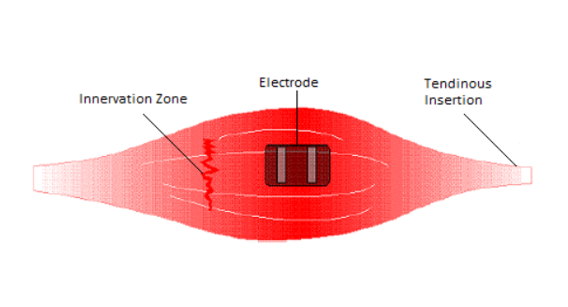
\includegraphics[scale=0.8]{imagenes/EstadodelArte/electrodo.png}
	\caption{Posición de los electrodos}
	\label{fig:Posici}
\end{figure}
 

El kit biosignalplux nos va a permitir adquirir las señales EMG y poder ver la interacción eléctrica en tiempo real. Este kit será el que utilicemos para obtener las señales EMG y procesarlas posteriormente.




